\chapter{总结}
\label{chap:summary}

\section{用户反馈}

\subsection*{优点}
\noindent\textbf{1. AI 交友推荐较为精准，容易找到共同话题。}
可以用自己的话填写兴趣和交友偏好。推荐卡把人物自述、兴趣标签和参考契合度放在一起，容易看出对方哪里吸引自己。
例如，期待结识喜欢自然、愿意分享日常的人时，林澈卡片上的“喜欢旅行”“喜欢自然”，以及她想和朋友一起发现路边风景的自述，都能与这份期待对应起来。看完就能想到第一张纸条可以问什么，
比如“最近散步时，有没有遇到值得停下来看一眼的风景？”

\begin{figure}[H]\centering
  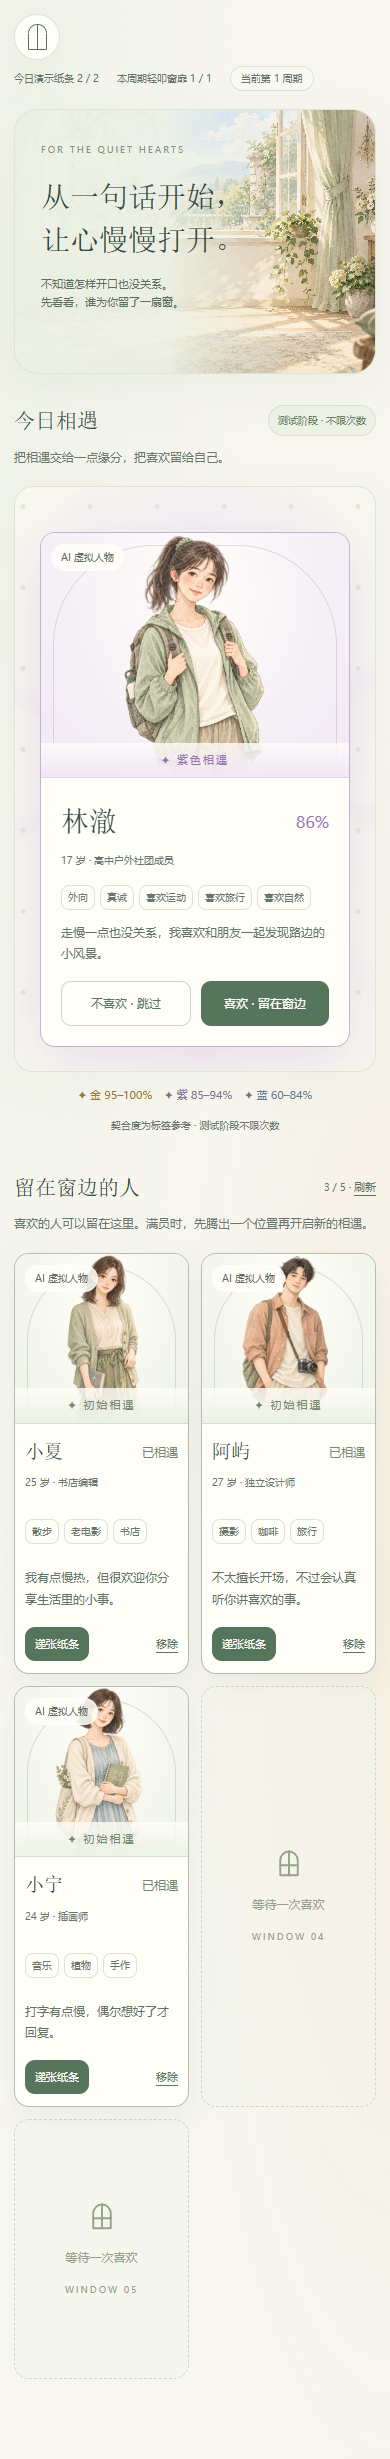
\includegraphics[viewport=40 1483 351 1679,clip,height=25mm]{assets/report/feedback/draw-purple-390.png}
  \caption{推荐卡片上的参考契合度、兴趣标签和人物自述}
\end{figure}

\noindent\textbf{2. AI 生成的回复多样，也能启发自己的表达。}
对方说，读完书中描写山间散步的段落，很想出去走走。面对同一句话，可以聊文字本身，用“那段描写一定很有画面感”接住对方的感受；
也可以问“你平时也喜欢去山里走走吗”，把话题从书带到生活；还可以用一句关于散步计划的玩笑让语气轻松一些。
即使一条都没选，也可能因此想起自己走过的山路，写下一句更像自己的回答。

\begin{figure}[H]\centering
  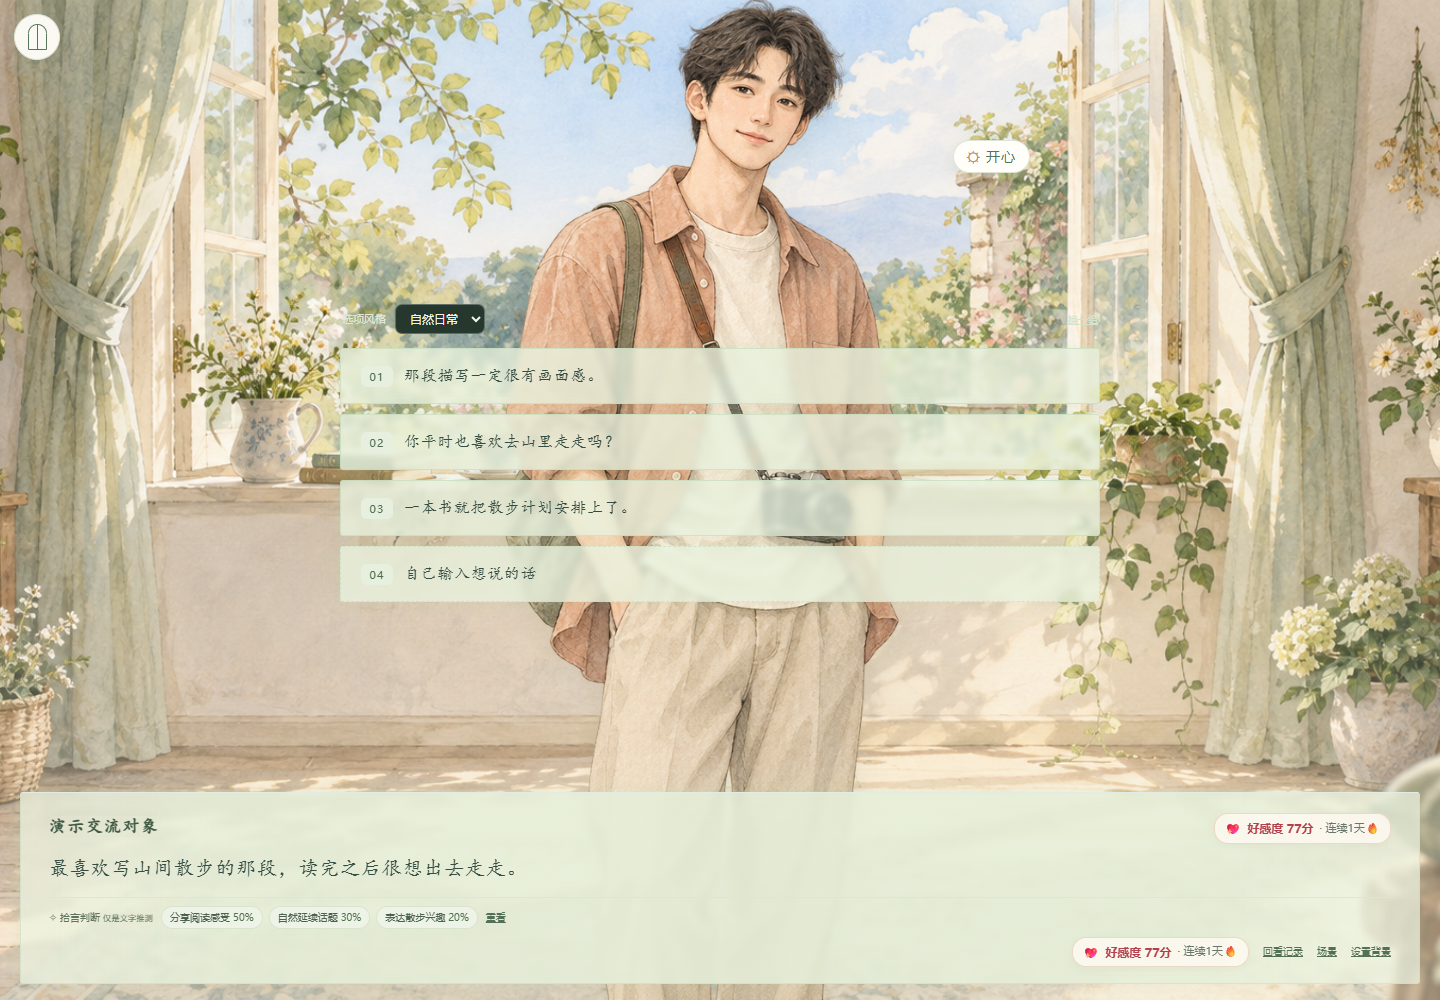
\includegraphics[viewport=334 395 1106 656,clip,width=.69\linewidth]{assets/report/chat.png}
  \caption{围绕同一句阅读感想给出的三种回复，以及手动输入入口}
  \label{fig:summary-chat}
\end{figure}

\clearpage
\noindent\textbf{3. 背景和界面优美典雅，画面能呼应交流的节奏。}
首页把进入应用设计成推开一扇窗：浅色背景中只有窗景、标题和一句邀请，留白给人慢慢走近的感觉。进入对话后，
水彩笔触和柔和配色延续下来，窗后的远景可以换成游乐园等更贴合心情的场景。人物站在画面中央，台词和回复选项落在半透明的浅色面板上，
读字时仍看得见身后的景物。从开窗时的安静，到与人交谈时的生动，两个页面各有气氛，也都呼应了项目里那句“让一句问候慢慢开始”。

\begin{figure}[H]\centering
  
\includegraphics[viewport=430 125 1010 769,clip,height=55mm]{assets/report/feedback/desktop-entry.png}\hspace{7mm}
  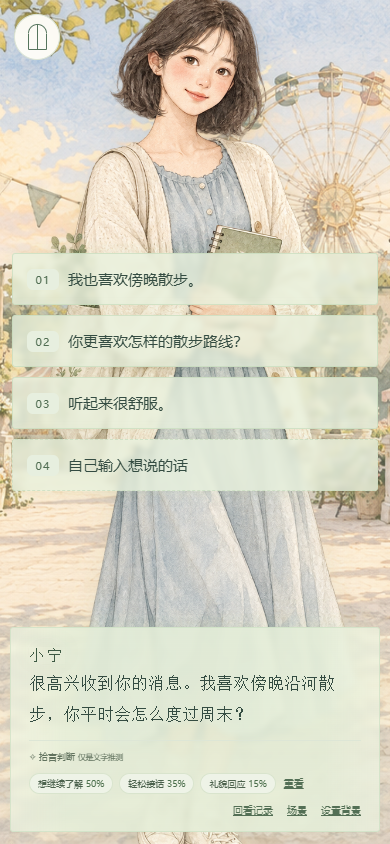
\includegraphics[height=55mm]{assets/report/feedback/date-scene-390.png}
  \caption{开窗入口的留白与窗景（左），游乐园对话中的水彩立绘与文字面板（右）}
\end{figure}

\subsection*{不足}
\noindent\textbf{1. AI 对言外之意的解读偏简单。}
图中把一句问候归为“分享心情”“自然接话”和“希望确认”等倾向，能提供一个粗略的阅读方向。真正让人拿不准的往往是另一类话：
朋友说“你可真行”，究竟是在真心称赞，还是对刚发生的事有些埋怨？当前的服务难以提供真正精准的分析，提供的实际帮助相当有限。

\begin{figure}[H]\centering
  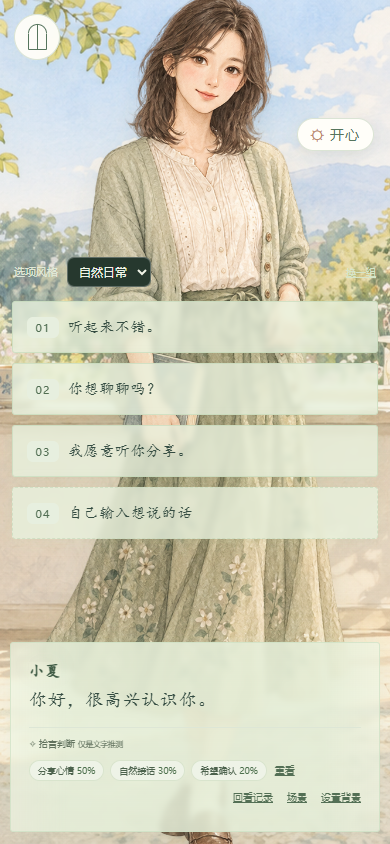
\includegraphics[viewport=8 33 379 202,clip,width=.57\linewidth]{assets/report/feedback/demo-390.png}
  \caption{一条问候下方的“拾言判断”以意图标签和占比呈现解读}
\end{figure}

\clearpage
\noindent\textbf{2. 手机端信息密集，操作时难以兼顾上下文。}
在 320 像素宽的对话页上，立绘、回复选项、消息正文和底部操作要共享同一屏。挑选回复时，
视线需要在选项和下方原话之间来回移动。纸条页则把真人纸条、虚拟来信、分类和操作按钮纵向排列，
一封来信的正文和回信按钮已经落在首屏以下。手机端可以优先展示当前消息和最常用的操作，让人物装饰和次要分类按需展开。

\begin{figure}[H]\centering
  
\includegraphics[height=68mm]{assets/report/feedback/revised-chat-320.png}\hspace{9mm}
  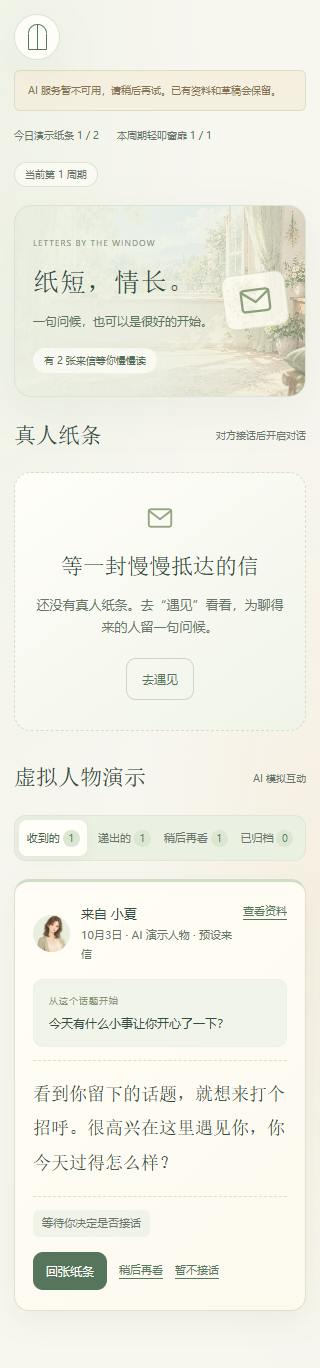
\includegraphics[height=81mm]{assets/report/feedback/letters-320.png}
  \caption{320 像素宽的对话首屏（左）与需要纵向滚动的纸条整页（右）}
\end{figure}

\noindent\textbf{3. 聊天停了一段时间后，缺少再次联系的契机。}
纸条被接住以后，用户可以随时从“进入真人对话”回到原来的会话。但隔了几天，即使还记得对方提过的那本书，
也可能因为担心打扰而迟迟没有开口。保留会话入口解决了“去哪里找人”，仍留下“现在说什么才自然”的难题。
如果用户能从上次交流里选一个愿意再聊的话题，自行决定何时发出问候，就更容易把一次愉快的聊天延续下去。

\begin{figure}[H]\centering
  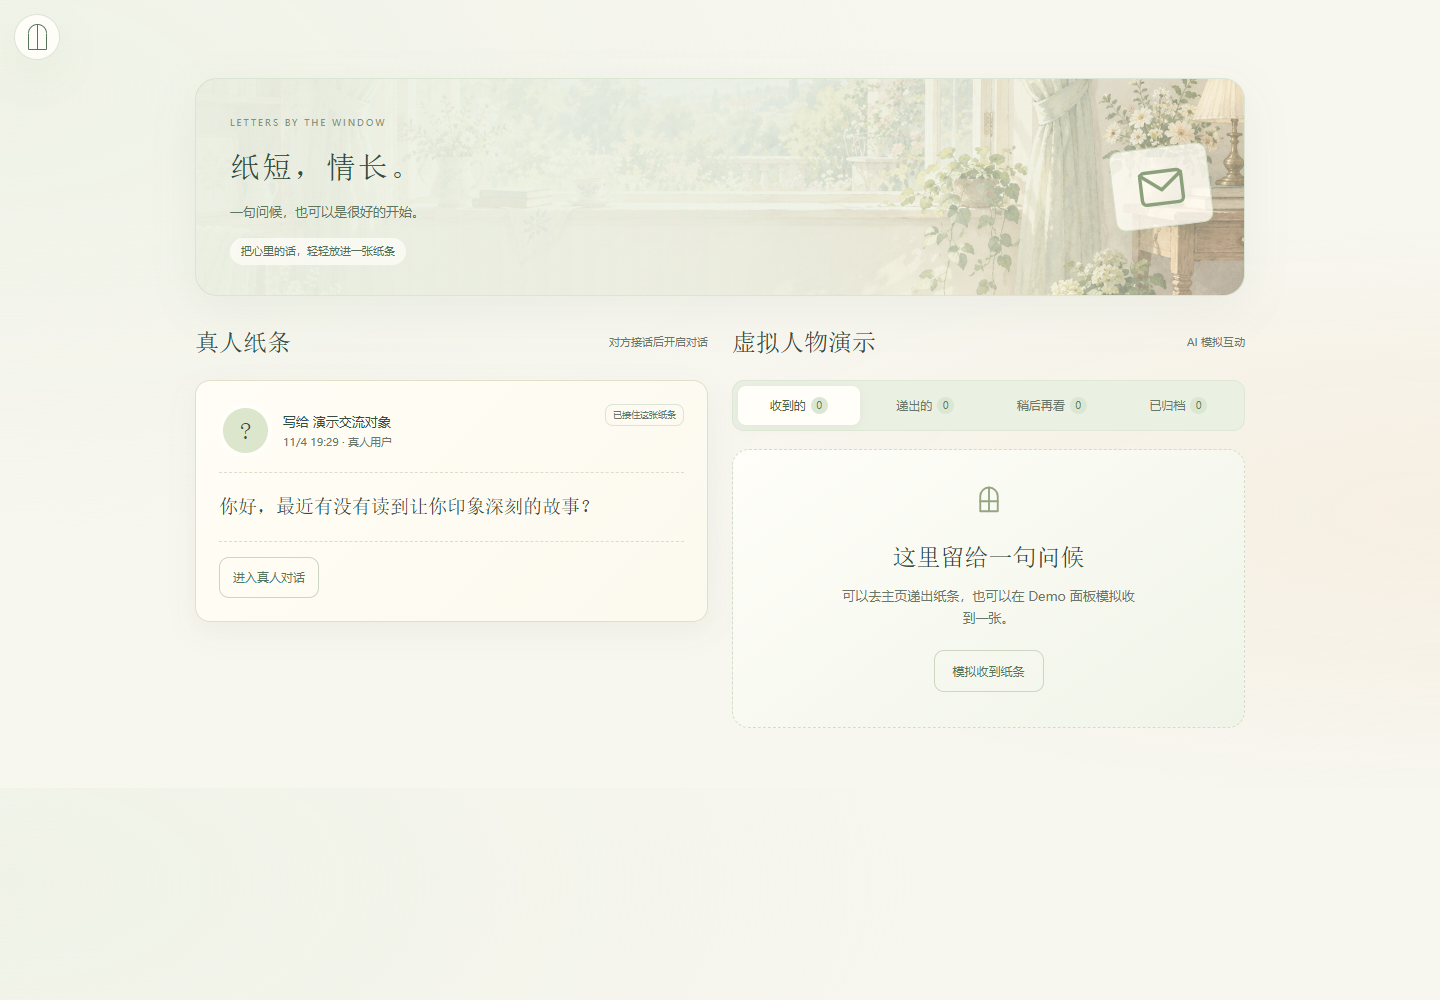
\includegraphics[viewport=185 370 717 677,clip,height=38mm]{assets/report/notes.png}
  \caption{已接住的纸条保留了最初的阅读话题和返回原会话的入口}
  \label{fig:summary-note}
\end{figure}

\clearpage
\section{项目总结}

人与人之间的距离，有时并非隔着山海，而是隔着一句尚未说出口的问候。
即使遇见兴趣相投的人，也可能因不知如何开口、难以揣摩对方的心意，
而让一段本可以发生的相识悄然止步。
“谁能打开你的窗”便从这份微小而真实的社交困境出发，
围绕从初次相遇到逐渐熟悉的过程，完成了需求分析、系统设计、开发与测试，
最终交付了一套可在浏览器中使用的低压力社交应用。
项目尝试以共同兴趣搭建相遇的契机，以双向意愿守护交往的边界，
再以适度的智能辅助与富有温度的交互设计，
让每一次主动靠近都不必仓促，让每一份回应都出于自愿。

\begin{enumerate}
    \item \textbf{以兴趣为引，让相识始于从容。}

    相识始于契机，相知则需要时间。
    共同的兴趣与相近的交友偏好，能够让两个原本陌生的人发现彼此的共鸣，
    却不足以替他们决定是否愿意走近。
    因此，系统将发现对象与建立联系分为两个循序渐进的阶段：
    以兴趣为线索寻找可能志趣相投的人，
    再以一张简短的纸条传递初次问候。
    纸条既是一次轻轻的叩窗，也是一份不必立即作答的邀请。
    发起者得以真诚表达结识的愿望，
    收到纸条的人则保有了解、思考与选择的余地。
    从发现彼此的相似，到确认双方的意愿，
    联系的建立不再依赖单方面的热情，
    而是在相互尊重中自然发生。
    如此，愿意迈出第一步的人可以勇敢尝试，
    习惯慢慢熟悉的人也无需匆忙回应。

    \item \textbf{以智能为辅，让表达不失本真。}

    有时，交流的阻碍并非无话可说，而是心中有意，笔下无言。
    面对已经建立的对话，系统借助 AI 理解当前的交流语境，
    为用户提供多种自然的接话思路，
    帮助那些一时词穷的心意找到恰当的表达。
    这些建议并非预先写好的标准答案，
    而是可供选择、借鉴或舍弃的参考。
    用户既可以从中获得启发，也可以沿着自己的思路自由回应。
    与此同时，虚拟人物互动提供了一个能够反复尝试的练习空间，
    让用户在真实交流之外探索不同的表达方式，
    逐渐找到适合自己的沟通节奏。
    智能技术在此并非代替人说话，而是帮助人更自在地说出自己的话。
    当交流真正发生于两个人之间，
    每一条消息的发送权仍然属于用户本人，
    每一次对话的进退也始终由双方共同决定。

    \item \textbf{以形色为媒，让情绪跃然屏间。}

    文字能够传递言语，却未必能够完整承载言语背后的神态与温度。
    隔着屏幕，同一句问候可能被读出不同的语气，
    同一份善意也可能因缺少表情而产生误解。
    为了让文字交流拥有更丰富的感知线索，
    系统在真人对话中引入人物立绘、个性化场景与情绪提示。
    用户可以选择自己喜爱的人物形象，
    聊天双方也能够分别布置符合个人偏好的对话场景。
    当新的消息抵达，立绘旁简短的情绪提示为文字增添一层语气参照；
    若对方设置了相应的表情立绘，
    人物的神态也会随之变化，
    让原本隐于字里行间的情绪多了一种可感知的呈现。
    这些视觉线索并不试图替代真实的理解与沟通，
    而是为阅读者提供更多体会对方语气的可能。
    当言语仍有歧义时，真诚的询问与确认，
    始终是拉近彼此距离的重要方式。

    \item \textbf{以时光为笺，让心意渐次澄明。}

    有些心意，适合在相遇时记录，却未必需要在当下言明。
    一次愉快的交谈或许令人心生好感，
    但这份感受究竟意味着什么，
    往往要经过时间的沉淀才能慢慢看清。
    为此，系统在虚拟人物互动中设计了私人“心笺”与七日“回望”机制。
    用户可以将相处时的感受悄悄写入心笺，
    不必急于将一时的悸动化作明确的表态；
    待七日之后，再回望曾经留下的文字，
    重新审视这一阶段的心意，并自主决定是否将其揭晓。
    从即时记录到延时回望，
    系统为感受的萌生与心意的确认保留了不同的时间尺度。
    那些尚未想清楚的话，可以暂时留在纸上；
    那些经过思考依然真切的感受，也终将拥有被认真对待的机会。
    让表达不必仓促，让选择不受催促，
    正是这一设计希望给予慢热者的温柔余地。
\end{enumerate}

“相知无远近，万里尚为邻。”
从一张试探性的纸条，到一句逐渐自然的回应；
从屏幕间可感的情绪，到时光中慢慢明朗的心意，
“谁能打开你的窗”所探索的，
不仅是如何让陌生人建立联系，
更是如何让每个人在靠近他人时保有勇气，
在面对回应时懂得尊重，
在表达自我时拥有从容。
技术能够为相遇创造契机，
而真正推开那扇窗的，始终是人与人之间自愿而真诚的交流。

